
% vim:set ff=unix expandtab ts=2 sw=2:
%\begin{columns}[t,totalwidth=\wcols] % use for debugging
\begin{columns}[t]
  \begin{column}[t]{\wcolA}
    %% now draw the actual boxes
    % columnA
    %\begin{myBox}[\hboxOneA]{Beamer blocks}
    \begin{myBox}[\hboxOneA]{Beamer blocks}
      
% vim:set ff=unix expandtab ts=2 sw=2:
Since our poster template uses the beamer class,
we can influence the defaults for beamer blocks by the template.
(for example the background and foreground colors, fonts and fontsize for content and header of this box)
Which can help to avoid a lot of formatting in the user code andmakes it easier to achieve a standard layout.
The interior is quite flexible.\\
\begin{itemize}
	\item we add a pseudo picture
\end{itemize}
	\begin{figure}[tb]
		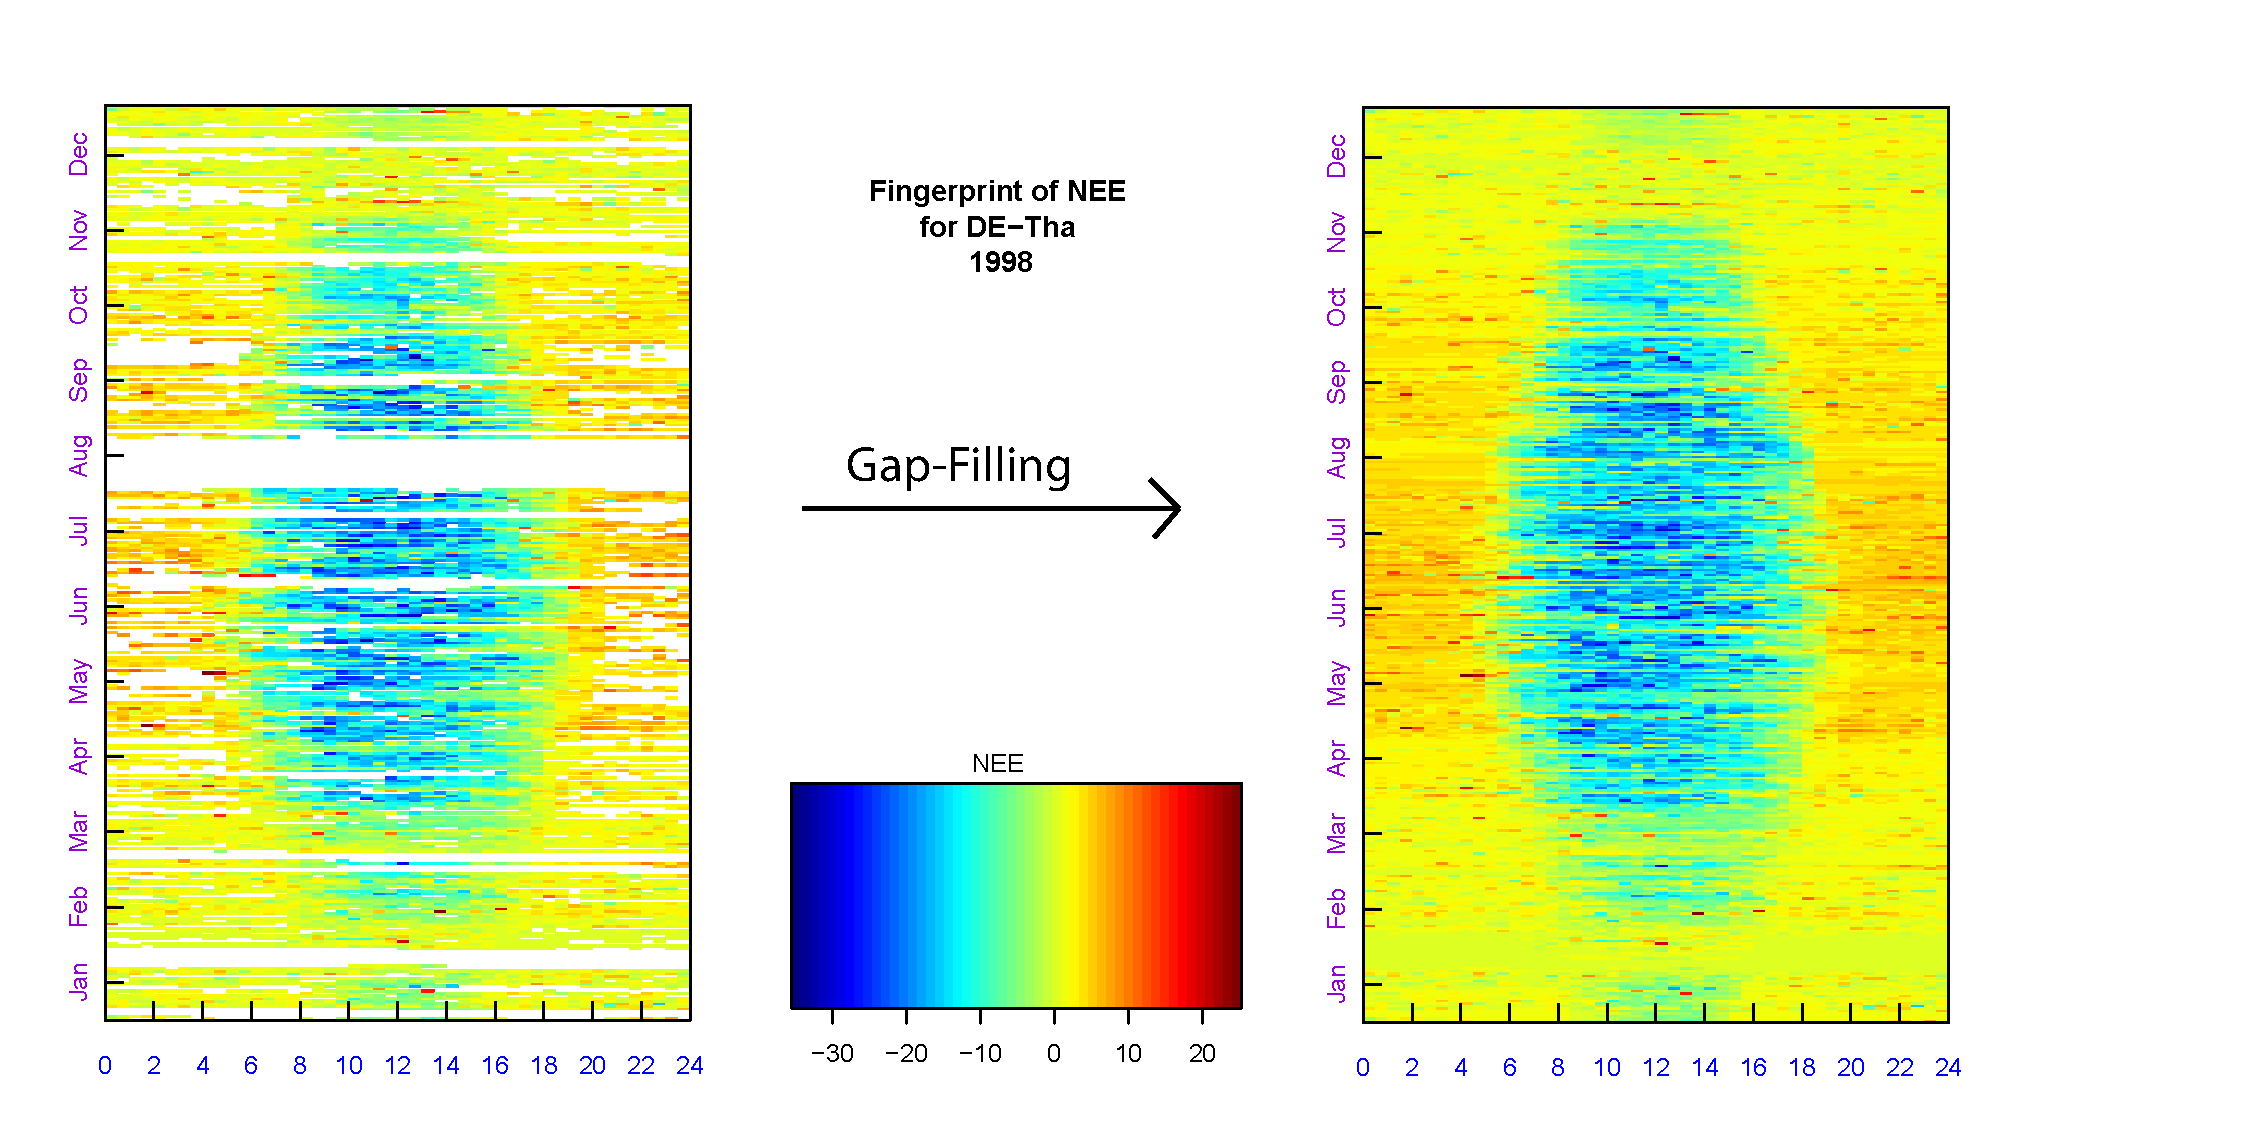
\includegraphics[height=3cm]{images/content/DE-Tha_1998_FP_NEE_ffc.pdf}
    \caption{a pseudo caption}
	\end{figure}




    \end{myBox}
    \vspace{\vblocksep}  
    \begin{myBox}[\hboxTwoA]{Vertical alignment hack}
      
% vim:set ff=unix expandtab ts=2 sw=2:
Beamer boxes can be used inside the columns environment, also provided by the beamer class.
This simplifies some common vertical and horizontal alignment tasks.
\alert{However there is one notable exception that requires a hack:}\\

It is not possible to directly align beamer blocks vertically 
at the top \alert{AND} the bottom of the poster simultaneously for the following reason.
The block environment has no \emph{height} parameter. 
The blocks grow with their content and the header.
We can influence there size only indirectly by wrapping their content in minipages.
The following code defines a minimal environment that allows 
to add extra white space to the blocks.
\inputminted{latex}{content/myBox.tex}
With control over the vertical extent established, we can choose the size of the first box in a column and then use
\LaTeX2e s built in computing facilities (
  \verb1 \dimexpr1 and \verb1 \numexpr1) to determine the size of the second box.
\inputminted{LaTeX}{content/lengths.tex}



    \end{myBox}
  
  \end{column}
  
  %% column specific
  %% colB
  % compute the width of the second column 
  \newlength{\wcolB}
  \setlength{\wcolB}{\dimexpr \wcols-\wcolA \relax} 
  
    \begin{column}[t]{\wcolB}
    \newlength{\hboxOneB}
    % This time we even go a step further and measure
    % the contents of the first box before we draw it
     \newsavebox\myMeasuringBox
      \savebox{\myMeasuringBox}{
      \begin{myMiniPage}%
        
% vim:set ff=unix expandtab ts=2 sw=2:
  {\vspace{.2cm}\textbf{REddyProc}\hfill\normalsize{her could be some names}}
\alert{\textit{Context:}}

To measure how much space this box will take we put it in a 
savebox:


      \end{myMiniPage}%
    }
      \setlength{\hboxOneB}{\ht\myMeasuringBox}% height (above baseline) 
      \addtolength{\hboxOneB}{\dp\myMeasuringBox}% and depth (below baseline) of the box 

    % compute the height of the second box 
    \newlength{\hboxTwoB}
    \setlength{\hboxTwoB}{ \dimexpr ( \hcols - \hboxOneB) \relax}
    
    \begin{myBox}[\hboxOneB]{Measured block}
      \usebox{\myMeasuringBox}
    \end{myBox}
    \vspace{\vblocksep}  
    \begin{myBox}[\hboxTwoB]{Conclusions}
      
% vim:set ff=unix expandtab ts=2 sw=2:
Here is the code used to produce these two columns


    \end{myBox}
  \end{column}
\end{columns}
